\documentclass{report}
\usepackage[english]{babel}
\usepackage[letterpaper,top=2cm,bottom=2cm,left=3cm,right=3cm,marginparwidth=1.75cm]{geometry}
\usepackage{amsmath}
\usepackage{graphicx}
\usepackage{listings}
\usepackage{amssymb}
\usepackage[colorlinks=true, allcolors=blue]{hyperref}
\usepackage{float}
\usepackage{listings}
\usepackage{color}

\setcounter{tocdepth}{4}
\setcounter{secnumdepth}{4}

\definecolor{dkgreen}{rgb}{0,0.6,0}
\definecolor{gray}{rgb}{0.5,0.5,0.5}
\definecolor{mauve}{rgb}{0.58,0,0.82}

\lstset{frame=tb,
  language=Java,
  aboveskip=3mm,
  belowskip=3mm,
  showstringspaces=false,
  columns=flexible,
  basicstyle={\small\ttfamily},
  numbers=none,
  numberstyle=\tiny\color{gray},
  keywordstyle=\color{blue},
  commentstyle=\color{dkgreen},
  stringstyle=\color{mauve},
  breaklines=true,
  breakatwhitespace=true,
  tabsize=3
}

\graphicspath{{images}}

\title{Playing with 3D equations and planes/graphs}

\author{Mr Ashlin Darius Govindasamy\\ \large{University of South Africa}}

\date{\today}

\begin{document}
\maketitle
\newpage

\tableofcontents

%for adding page numbers
\pagenumbering{arabic} 

\chapter*{Introduction}
%add subsections like this
\subsection{Hello World}
This is a template to get started in writing papers or scientific reports.

\chapter{Graphing lines and equations in 3D space using software}
Why graph in 3D? In school or universities they dont actully make you draw the 3D graph or teach you that (thats because during examinations you use just pen and paper and methodolgy to solve the problem no access to the computer). But in real life, you can use the computer to draw the 3D graph in seconds to give you a picture of your function.

When playing or calculating with functions i would like to see what that function is doing in 3D. This is a good way to see what the function is doing in 3D. For example finding a plane in 3D perpendicular to a point in 3D space or to another 3D plane. The way universites tell you check if your equations is correct is to prove it mathematically using some concrete methodolgy or theorem. This is a good way to prove your equations are correct.
I believe that a much easier way to prove your equations is to graph them in 3D and it looks more cooler to visualize them it also gives you a better idea/understanding of what the function is doing in 3D.

So when I am going to explain the 3D planes in the next chapter I will use the following software to graph the 3D planes to give you a picture on what is happening. For now im going to explain free software graphing methodologies so you can plot any 3D functions.

\subsection{Graphing with the Python (Matplotlib library)}

Python is a high-level, interpreted, general-purpose programming language. Its design philosophy emphasizes code readability with the use of significant indentation. Python is dynamically-typed and garbage-collected.
We will use the python language with the language a package called matplotlib. This package is a collection of several plotting libraries. It is endorsed by Matlab but Matlab is paid the stuff i am showing your is free.


\begin{figure}[htb]
\centering

\includegraphics[width=0.15\textwidth]{python.png}
\caption{Python Programming Language Logo}
\label{fig:python}
\end{figure}

\begin{figure}[htb]
\centering
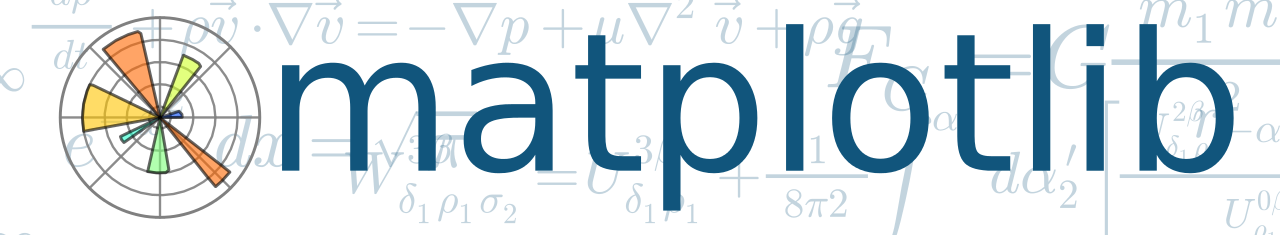
\includegraphics[width=0.25\textwidth]{matplotlib.png}
\caption{Matplotlib Logo}
\label{fig:matplotlib}
\end{figure}
    
\subsubsection{Setting up environment}

First you need to install Python. This is done by opening a terminal and typing the following:
Note this is for linux users.
\begin{lstlisting}[language=bash]
sudo apt-get install python3    
sudo apt-get install python3-pip
\end{lstlisting}

For windows users, you can download the python installer from here: https://www.python.org/downloads/ or install it using the windows store.

Then you need to install the matplotlib package. This is done by typing the following:
\begin{lstlisting}[language=bash]
pip install matplotlib
\end{lstlisting}

pip or pip3 depending on the pip you got ...

If you are struggling check out some tutorials on YouTube on Python or do a course on it.

\subsubsection{Python Demo plotting 3D Graphs}
I have created this demo to showcase some 3D Graph sketching with Python + Matplotlib Library. I wont explain code but consider these examples as a starting point.
Consult the web for library documentation for certain functions being used in my code samples below.

Check out https://matplotlib.org/ for more information on the Matplotlib library.

\begin{lstlisting}[language=Python]
import numpy as np 
import matplotlib.pyplot as plt 
import mpl_toolkits.mplot3d

#plot 3d planes 2x+2y+3z=0 and 3x+5y+7z=0

#increase dpi
plt.rcParams['figure.dpi'] = 200
x = np.linspace(-5,5,100)
y = np.linspace(-5,5,100)
X,Y = np.meshgrid(x,y)
Z = 2*X+2*Y+3
fig = plt.figure()
ax = fig.add_subplot(111, projection='3d')
ax.plot_surface(X,Y,Z,alpha=0.2)
Z = 3*X+5*Y+7
ax.plot_surface(X,Y,Z,alpha=0.2)
### you can add more graphs here ... following this procedure
ax.set_title('2x+2y+3z=0 and 3x+5y+7z=0')
plt.show()
\end{lstlisting}

\begin{figure}[H]
\centering
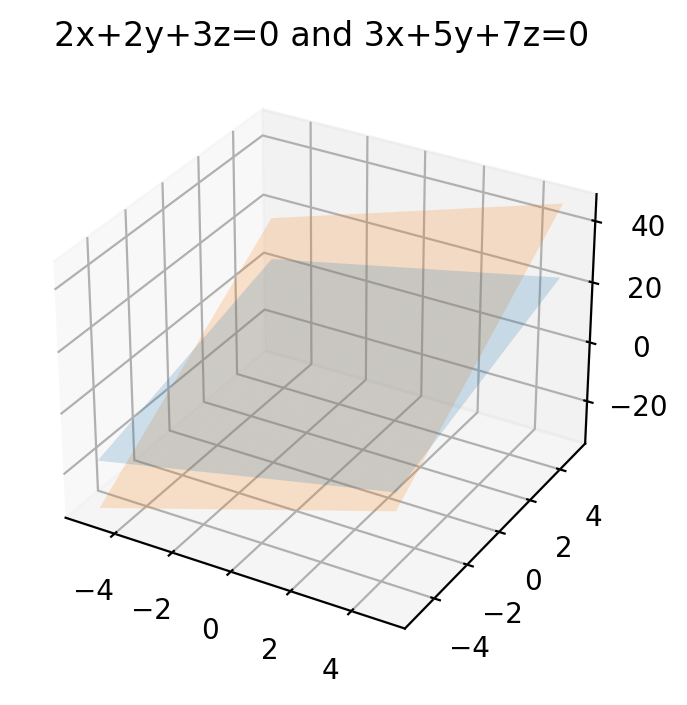
\includegraphics[width=0.5\textwidth]{output_1_0.png}
\caption{3D Graph of $2x+2y+3z=0$ and $3x+5y+7z=0$ generated with Matplotlib}
\label{fig:line3d}
\end{figure}

\begin{lstlisting}[language=Python]
import numpy as np 
import matplotlib.pyplot as plt 
import mpl_toolkits.mplot3d
#increase dpi
plt.rcParams['figure.dpi'] = 200
#plot 1/2*cos(x+y)
x = np.linspace(-5,5,100)
y = np.linspace(-5,5,100)
X,Y = np.meshgrid(x,y)
Z = 0.5*np.cos(X+Y)
fig = plt.figure()
ax = fig.add_subplot(111, projection='3d')
ax.plot_surface(X,Y,Z,alpha=0.2)
#show title
ax.set_title('1/2*cos(x+y)')
plt.show()
\end{lstlisting}    

\begin{figure}[H]
\centering
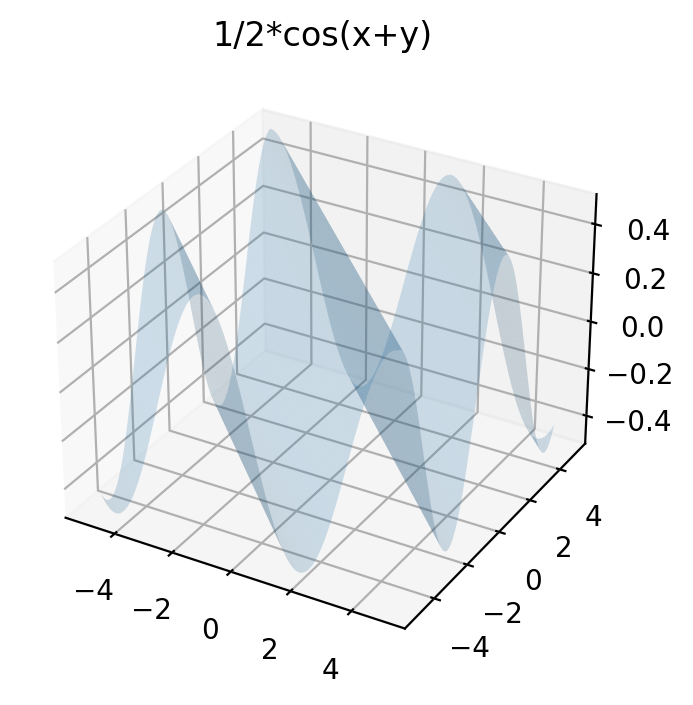
\includegraphics[width=0.5\textwidth]{output_2_0.png}
\caption{3D Graph of $\frac{1}{2}\cos(x+y)$ generated with Matplotlib}
\end{figure}

\begin{lstlisting}[language=Python]
def f(x, y):
    return np.sin(np.sqrt(x ** 2 + y ** 2))
#increase dpi
plt.rcParams['figure.dpi'] = 200
x = np.linspace(-6, 6, 50)
y = np.linspace(-6, 6, 50)
X, Y = np.meshgrid(x, y)
Z = f(X, Y)
fig = plt.figure()
ax = plt.axes(projection='3d')
ax.contour3D(X, Y, Z, 50, cmap='rainbow_r')
ax.set_xlabel('x')
ax.set_ylabel('y')
ax.set_zlabel('z')
#set title of equation
ax.set_title('sin(sqrt(x^2+y^2))')
plt.show()
\end{lstlisting}

\begin{figure}[H]
\centering
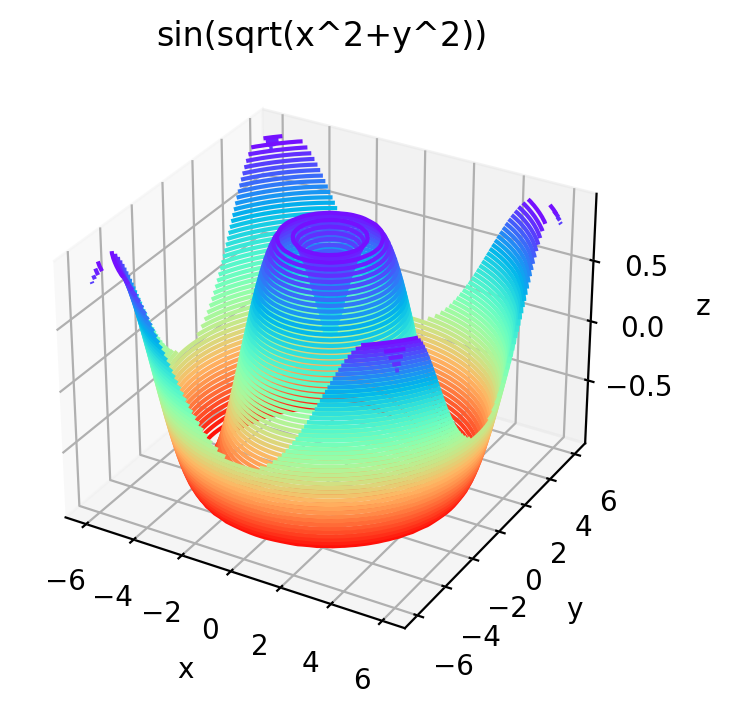
\includegraphics[width=0.5\textwidth]{output_3_0.png}
\caption{3D Graph of $\sin(\sqrt{x^2+y^2})$ generated with Matplotlib}
\end{figure}

\newpage

\begin{lstlisting}[language=Python]
import numpy as np 
import matplotlib.pyplot as plt 
import mpl_toolkits.mplot3d

#increase dpi
plt.rcParams['figure.dpi'] = 200

#plot x^2+2y+5=0 in 3d
x = np.linspace(-5,5,100)
y = np.linspace(-5,5,100)
X,Y = np.meshgrid(x,y)
Z = X**2+2*Y+5
fig = plt.figure()
ax = fig.add_subplot(111, projection='3d')
ax.contour3D(X,Y,Z,50,cmap='twilight_shifted')
#show title
ax.set_title('x^2+2y+5=0')
plt.show()
\end{lstlisting}
\begin{figure}[H]
\centering
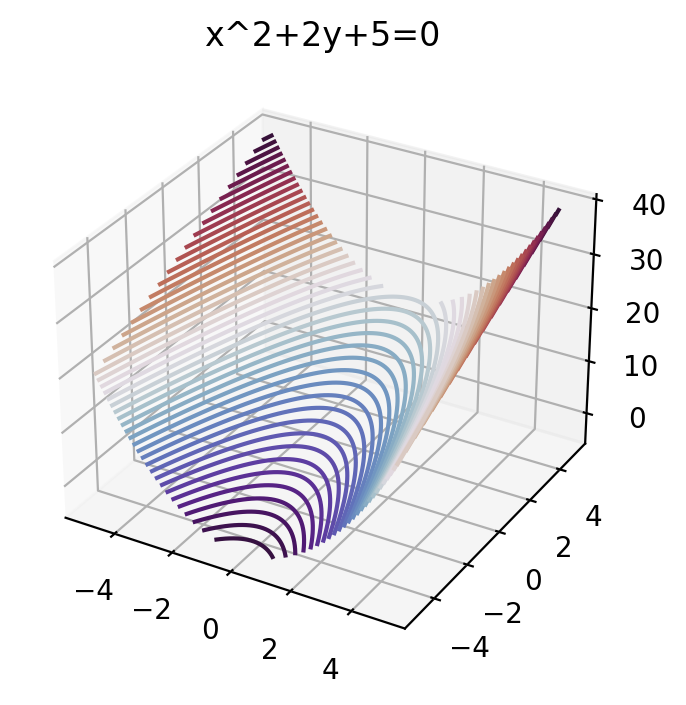
\includegraphics[width=0.5\textwidth]{output_4_0.png}
\caption{3D Graph of $x^2+2y+5=0$ generated with Matplotlib}
\end{figure}

\newpage
From manpulating my code you could easily explore and graph any function you desire. You can be creative with the colors, shapes, and sizes of the graphs.
If you want to just play around have fun! I hope you enjoy my demo and code sample.

This library is so powerful you can do anything possible with it the creativity and research is up to you.




\newpage

\subsection{Graphing with Geogebra (Online Web Platform)}
For the purposes of this paper, we will use the Geogebra Web Platform. This is a free online platform that allows you to graph 3D graphs and equations. You dont need to be logged in to use this platform or install anything on your computer. This is a website/cloud platform.
GeoGebra is an interactive geometry, algebra, statistics and calculus application, intended for learning and teaching mathematics and science from primary school to university level. GeoGebra is available on multiple platforms, with apps for desktops, tablets and web.

%insert figure
\begin{figure}[htb]
\centering
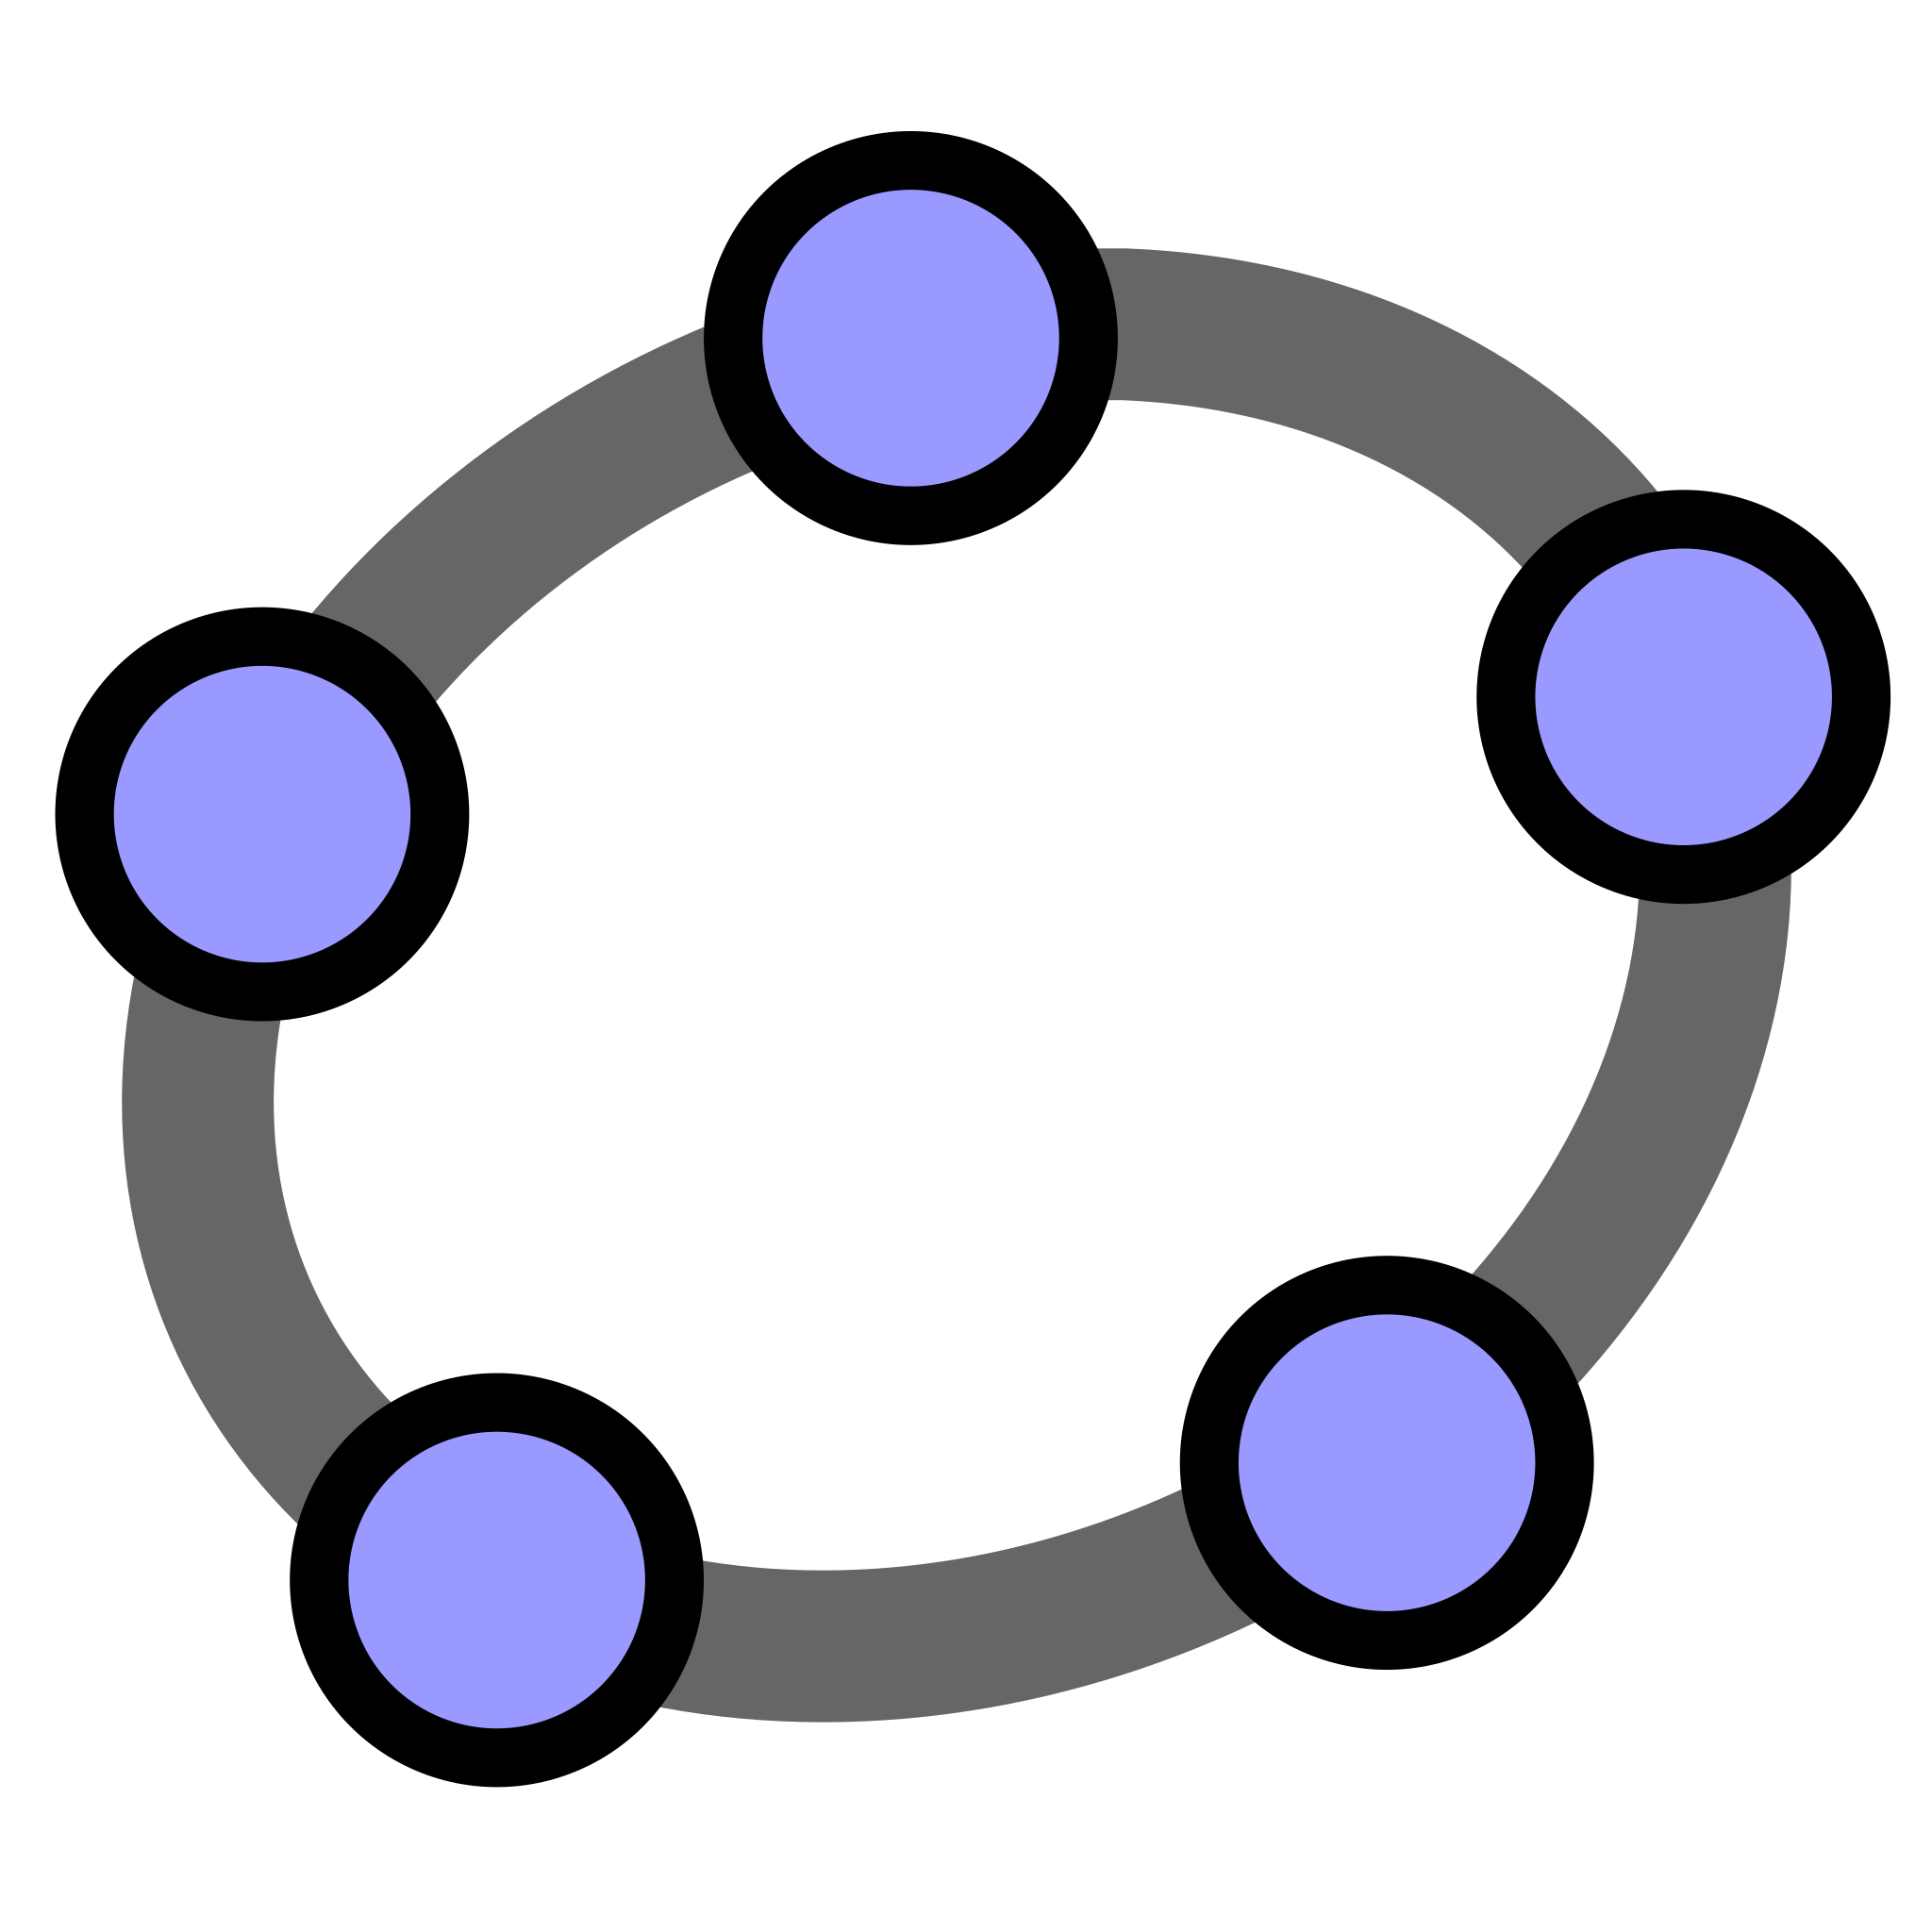
\includegraphics[width=0.4\textwidth]{geogebralogo.png}
\caption{GeoGebra Logo}
\label{fig:geogebra}
\end{figure}



\subsubsection{Our first Geogebra session}

To get started with Geogebra, we will first create a new Geogebra workspace. This is done by opening a new Geogebra window which is followed by going to this link:
https://www.geogebra.org/3d?lang=en

it would look like this below:
\begin{figure}[htb]
\centering
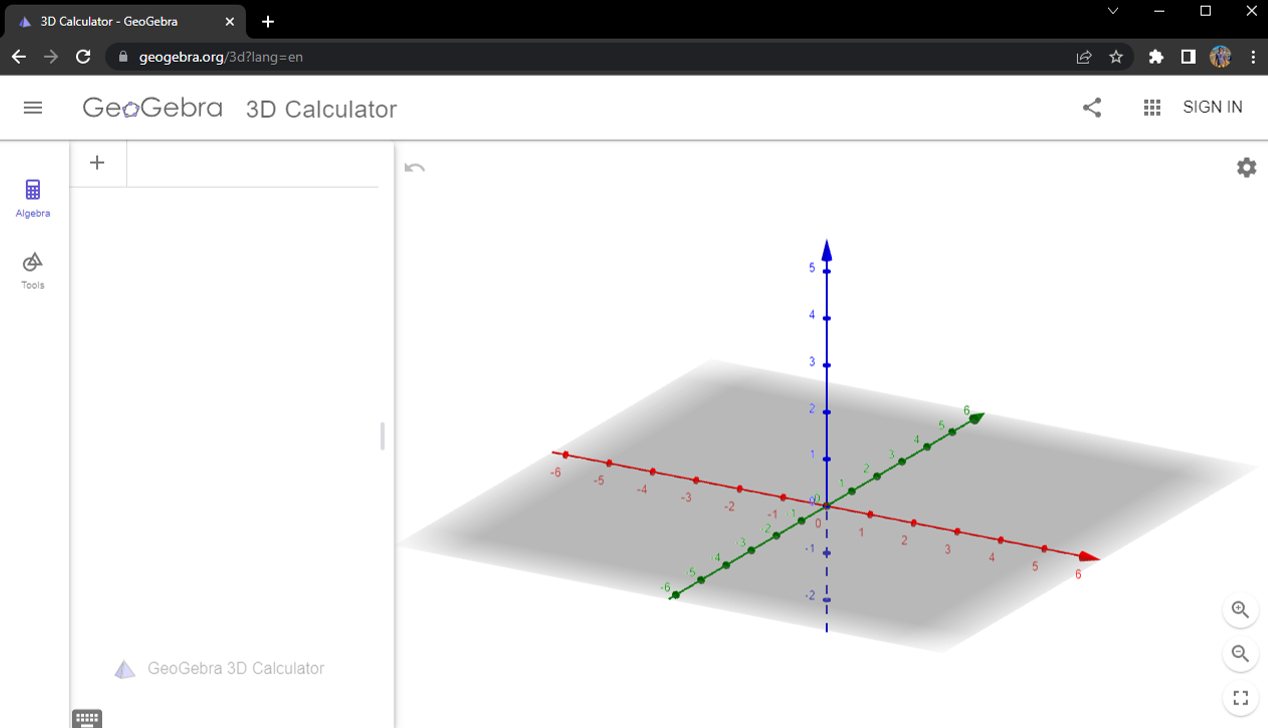
\includegraphics[width=0.9\textwidth]{geogebra.png}
\caption{GeoGebra Workspace}
\label{fig:geogebraworkspace}
\end{figure}

You can now get started with graphing.

For additional things to do check out the tools in the tools tab. It looks like something like this.
\begin{figure}[htb]
\centering
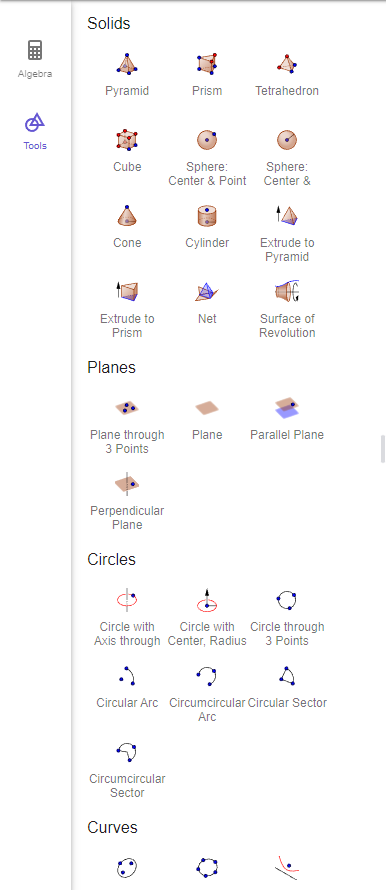
\includegraphics[width=0.4\textwidth]{tools.png}
\caption{GeoGebra Tools}
\label{fig:geogebratools}
\end{figure}

The way you learn is by experimenting have fun!

\newpage

\subsubsection{Plotting equations and vectors}
To plot any equation just type it in the Geogebra workspace. And for plotting a point in the 3D space. Just express your vector as a tuple of coordinates.

In this diagram i have plotted some 3D equations and vectors.

\begin{figure}[htb]
\centering
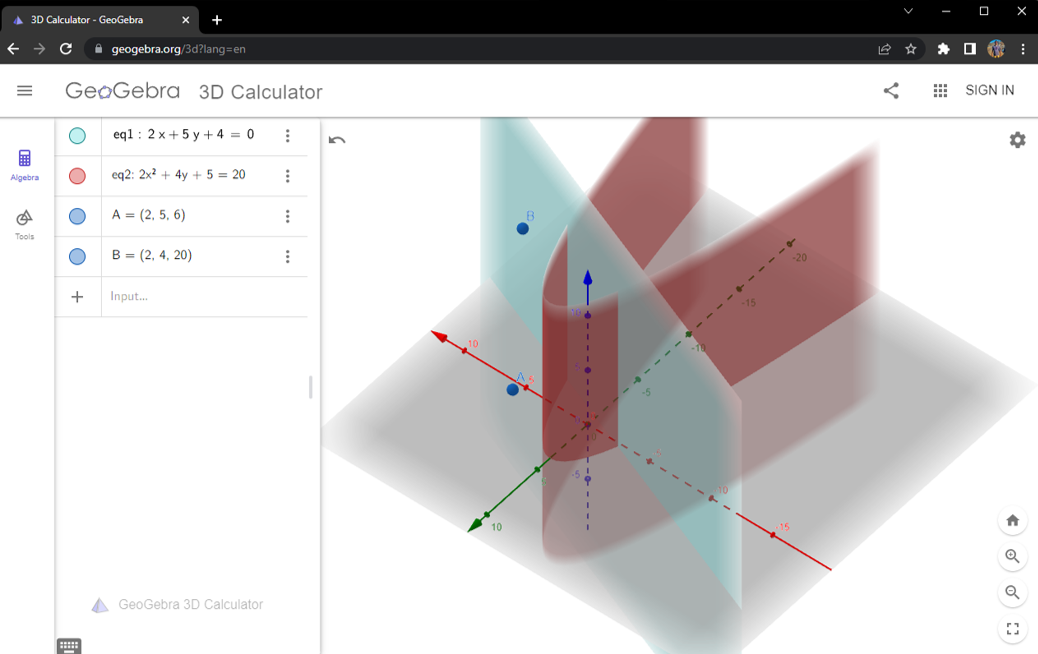
\includegraphics[width=0.8\textwidth]{3d-graph.png}
\caption{GeoGebra Workspace with Equations and Vectors}
\label{fig:geogebragraphs}
\end{figure}



\chapter{Lines and Planes in 3-Space}
\subsection{Equations of lines and planes in 3-space}

\subsubsection{Equations of planes}

Consider the following equations:

\begin{center}
    \begin{tabular}{ | c | }
        \hline
        \textbf{Equations of planes in 3-space}             \\ \hline
        Point-normal: $a(x-x_0) + b (y-y_0) + c(z-z_0) = 0$ \\ \hline
        General Form: $ax + by + cz + d = 0$                \\ \hline
        Vector form: $n(r-r_0) = 0$                         \\
        or $(a; b; c)(x-x_0; y-y_0; z-z_0) = 0$             \\ \hline
    \end{tabular}
\end{center}

We note that in the equations above, $(a; b; c)$ is a vector perpendicular to the plane and $(x_0; y_0; z_0)$ is a
specific point on the plane.
Thus when we determine the equation of a plane we need to find, from the information
provided, a point on the plane and a vector perpendicular to the plane.

\subsubsection{Equations of lines}

Consider the following equations:

\[ L_n
\begin{cases} 
x = x_0 + at \\ 
y = y_0 + bt & -\infty < t < \infty \\ 
z = z_0 + ct \\
\end{cases} 
\]

This equation represents parametric line equations in 3D space alternatively, we can write this equation in the following vector form:

\begin{center}
$r = r_0 + vt ,$ $ -\infty < t < \infty$ \\
or $(x,y,z) = (x_0+y_0+z_0)+(a,b,c)t$ 
\end{center}


We note that in the equations above, $(a; b; c)$ is a vector parallel to the line and $(x_0; y_0; z_0)$ is a specific
point on the line.
Thus when we determine the equations of a line we need to find, from the information
provided, a point on the line and a vector parallel to the line.
The important point to notice here is that when we are finding the equation
of a plane we need a vector perpendicular to the plane, and when we are
finding the equations of a line we need a vector parallel to the line.


\subsection{Determining the properties of planes and methodologies to prove them}
\subsubsection{Finding out if the planes are parallel or perpendicular/Orthogonal to each other}
\textbf{Procedure for testing perpendicular/Orthogonality planes}\\
To get started in proving that the planes are perpendicular/orthogonal to each other. We need to find out our two $(a,b,c)$ vectors.
We take our two planes and find the $(a,b,c)$ vector of each plane. \\

With these two vectors work out if the dot product is = 0 or not. \\

Consider vectors $n,v$

Using this formula to calculate:

\begin{equation}
    \arccos{(\theta)}(\frac{u*v}{\| u\Vert \| v\Vert })
\end{equation}

we can deduct where dot product is:

$\left(n_1,\:\:\ldots ,\:\:n_k\right)\cdot \left(v,\:\:\ldots ,\:\:v_k\right)=\sum _{i=1}^kx_iy_i$ \\

If $\sum _{i=1}^kx_iy_i = $ 0, then the planes are perpendicular else if not 0, then the planes are not perpendicular. \\

\textbf{Procedure for testing parallel planes} \\

Consider the following plane equations:
\begin{center}
 $a_1x+b_1y+c_1z+d_1=0$ \\
 $a_2x+b_2y+c_2z+d_2=0$ \\
\end{center}

if 
\begin{center}
    $\frac{a_1}{a_2} = \frac{b_1}{b_2} = \frac{c_1}{c_2}$\\
\end{center}

then the planes are parallel \\

\subsection{Finding intersection of plane equations and if skew.}
Consider two lines:
\[ L_1
\begin{cases} 
x = x_0 + at \\ 
y = y_0 + bt \\ 
z = z_0 + ct \\
\end{cases} 
\]

and
\[ L_2
\begin{cases}
x = x_1 + dt \\
y = y_1 + et \\
z = z_1 + ft \\
\end{cases}
\]

we can find the intersection of these two lines by changing the $t$ letters in the line equations to make it different:
\[ L_1
\begin{cases}
x = x_0 + ar \\
y = y_0 + br & (1)\\ 
z = z_0 + cr \\
\end{cases}
\]

\[ L_2
\begin{cases}
x = x_1 + ds \\
y = y_1 + es & (2)\\
z = z_1 + fs \\
\end{cases}
\]

equate (1) and (2) and we get: \\
\[ S_1
\begin{cases}
x_0 + ar = x_1 + ds \\ 
y_0 + br = y_1 + es \\ 
z_0 + cr = z_1 + fs \\
\end{cases}
\]

solve for $s$ and $r$ once done then you subsitute the solved values in to any line equation to get the intersection point.

The same procedure will occur when dealing with general form equations. If there is no solution after you did the parallel check and also can not solve this system of equations thus, then the lines are skew.

\subsection{Finding the distance between a point and a plane}
Consider the distance between a point and a plane formula.

The distance from $(x_0,y_0,z_0)$ to the plane $Ax+By+Cz+D=0$ is: \\
\begin{equation}
    d = \frac{Ax_0+By_0+Cz_0+D}{\sqrt{A^2+B^2+C^2}}
\end{equation}

We can use this distance formula to find the distance between a point and plane.

\subsection{Worked Examples (Application)}
\subsubsection{Finding equation of plane that passes via 3 points}
Your problem statement is that you need to find the equation of a plane that passes through 3 points. \\ 

Consider the following points: \\

$P(2,1,4),Q(4,-2,7),R(5,3,-2)$ \\

First we need to get 2 vectors and find the normal ($n$) of it. \\ 

$a = \vec{PQ} = \left\langle 4-2,-2-1,7-4\right\rangle  = \left\langle 2,-3,3\right\rangle $ \\

$b = \vec{PR} = \left\langle 5-2,3-1,-2-4\right\rangle = \left\langle 3,2,-6\right\rangle $ \\

Our $n$ is described as the cross product of the two vectors $a$ and $b$: \\

$n = a\times b = \begin{pmatrix}2&-3&3\end{pmatrix}\times \begin{pmatrix}3&2&-6\end{pmatrix}$  \\

Cross product is given by: \\

$\left(u_1,\:u_2,\:u_3\right)\times \left(v_1,\:v_2,\:v_3\right)=\left(u_2v_3-u_3v_2,\:u_3v_1-u_1v_3,\:u_1v_2-u_2v_1\right)$ \\

$n = \begin{pmatrix}-3\left(-6\right)-3\cdot \:2&3\cdot \:3-2\left(-6\right)&2\cdot \:2-\left(-3\cdot \:3\right)\end{pmatrix}$ \\

$n = \begin{pmatrix}12&21&13\end{pmatrix}$ \\ 

Then we use the point $P$ to find the equation of the plane: \\

We will determine the equation of the plane by using the Point-Normal Format. \\

Our $(a,b,c) = (12,21,13)$ \\ 

and $(x_0,y_0,z_0) = (2,1,4) = P$ \\

Implementing the Point-Normal Format we get \\

$ 12(x-2)+21(y-1)+13(z-4)= 0 $ \\ 

expanded to: \\

$ 12x+21y+13z = 97$ \\

Below is the 3D graph of the plane to verify our solution.

\begin{figure}[H]
\centering
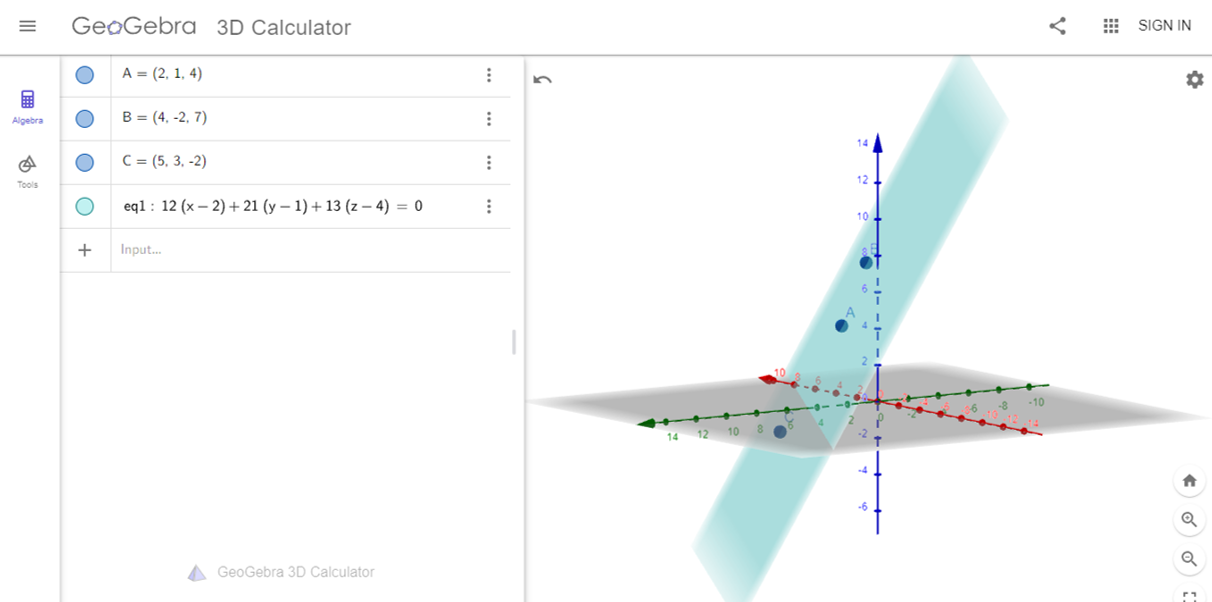
\includegraphics[width=1\textwidth]{3d-graph-worked(1).png}
\caption{3D Sketch of $12x+21y+13z = 97$ with points $P(2,1,4)$ and $Q(4,-2,7)$ and $R(5,3,-2)$}
\label{fig:Plane_3D_worked_1}
\end{figure}



\subsubsection{Finding out if 3 points are collinear in 3-Space}
Problem statement: Show that the points $A(1,2,3) , B(3,8,1), C(7,20,-3)$ are collinear. \\

Methodolgy: \\

First we need to find the vectors $\vec{AB}$ and $\vec{AB}$ and see if there is any relation/ratio between them.\\

$\vec{AB} = \left\langle 3-1,8-2,1-3\right\rangle = \left\langle 2,6,-2\right\rangle$ \\

$\vec{AC} = \left\langle 7-1,20-2,-3-3\right\rangle = \left\langle 6,18,-6\right\rangle$ \\

as you can see $\vec{AC} = 3\vec{AB}$ \\

$\therefore$ the points $A,B,C$ are collinear.

For fun let me show you how this looks in 3D.

\begin{figure}[H]
\centering
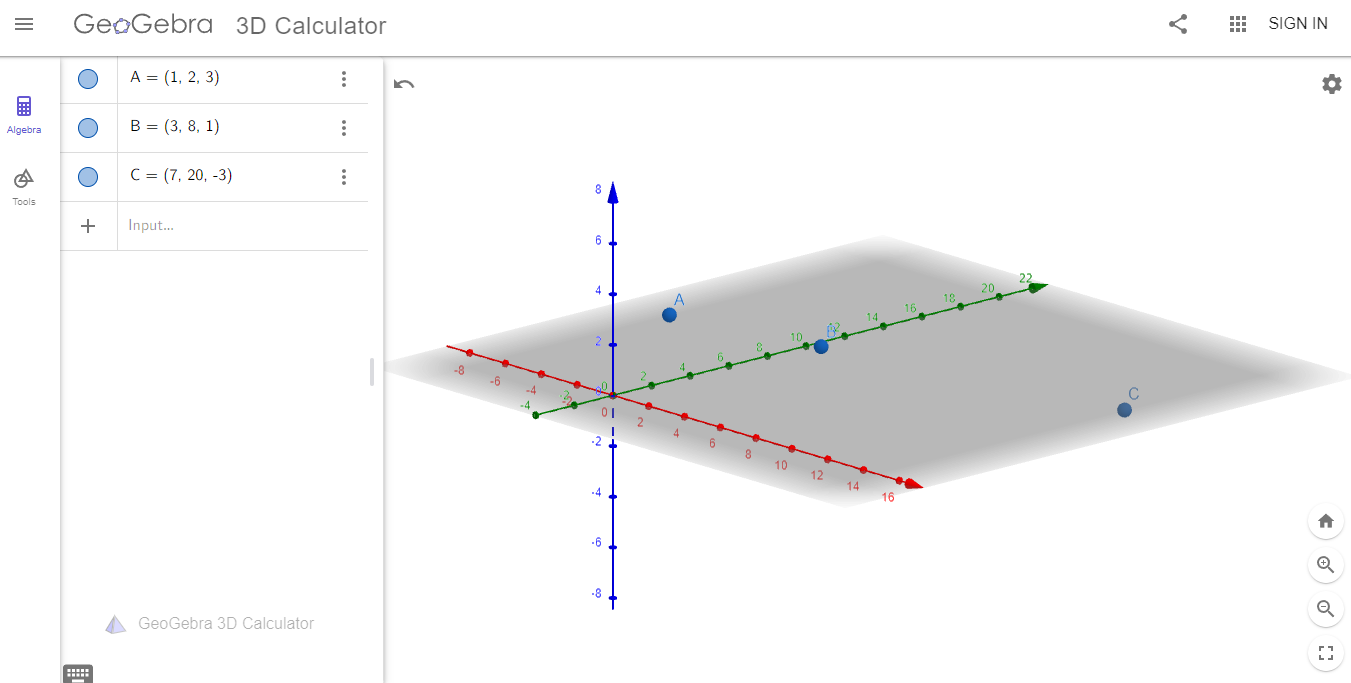
\includegraphics[width=1\textwidth]{3d-graph-worked(2).png}
\caption{3D Sketch of $A(1,2,3) , B(3,8,1), C(7,20,-3)$}
\label{fig:Plane_3D_worked_2}
\end{figure}

\subsubsection{Determining if two planes are parallel}
Problem statement: Determine if $L \land V$ are parallel. \\ 

Given: \\

\[ L
\begin{cases} 
x = 3t \\ 
y = 1+2t & -\infty < t < \infty \\ 
z = 2-t \\
\end{cases} 
\]

$V$ is a plane in 3-space defined by the equation: \\
\begin{center}
$V: 4x-y+2z=1$
\end{center}

Methodolgy: \\

Let $n = (4,-1,2)$ and $v = (3,2,-1)$ this is taken from the $(a,b,c)$ of the plane equations. \\

Since $L$ is a line in 3-space, $n$ is a normal of $V$ and we can consider $v$ parallel to $L$

\begin{figure}[H]
\centering
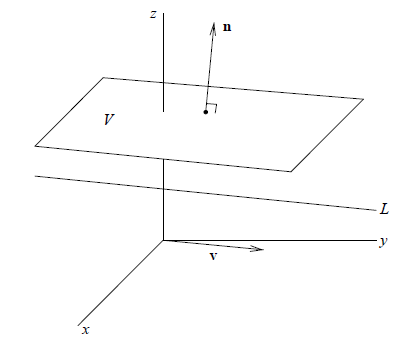
\includegraphics[width=0.5\textwidth]{sketch-3d-3.png}
\caption{3D Sketch of $L \land V$}
\label{fig:Plane_3D_worked_3}
\end{figure}

Now to find out if $V$ is parallel to $L$ we check if $n$ and $v$ dot product is 0 and perpendicular to each other. \\

$\vec{n}\cdot \vec{v} = (3,2,-1)*(4,-1,2)$ \\

$= 12-2-2 $ \\

$= 8$ \\

Hence $v$ is not perpendicular to $n$ and hence $L$ is not parallel to $V$.

\subsubsection{Finding the equation of a lane which contains a line and is perpendicular to another plane}
Problem statement: Find an equation for the plane $V_2$ which contains $L$ and is perpendicular to $V_1$:

Given: \\

\[ L
\begin{cases}
x = -1+3t \\
y = 5+2t & -\infty < t < \infty \\
z = 2-t \\
\end{cases}
\]

and $V_1$ is the plane in 3-space defined by: \\
\begin{center}
$V_1: 2x-4y+2z=9$
\end{center}

Procedure: \\

$L$ is given in vector form $(x,y,z) = (-1,5,2) + (3,2,-1)t$ \\ 

Hence $P = (-1; 5; 2)$ is a point on $L$ and $v = (3; 2;-1)$ is a vector parallel to $L$: Since $V_2$ contains $L$ it
follows that $P = (-1; 5; 2)$ is a point in $V_2$ and $v = (3; 2;-1)$ is parallel to $V_2$:
From the equation of $V_1$ it follows that a vector perpendicular to $V_1$ is $n_1 = (2;-4; 2)$ :
Since $V_1$ is perpendicular to $V_2$ it follows that $n_1 = (2;-4; 2)$ is parallel to $V_2$:

\begin{figure}[H]
\centering
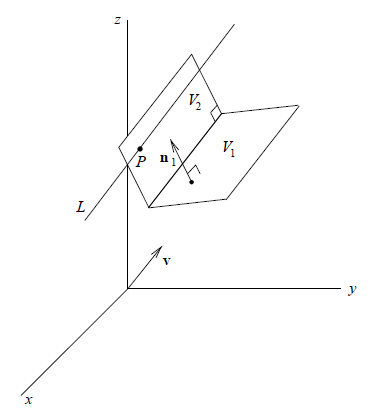
\includegraphics[width=0.5\textwidth]{sketch-3d-4.png}
\caption{3D Sketch of $L \land V_1 \land V_2$}
\label{fig:Plane_3D_worked_4}
\end{figure}

Thus $v$ and $n_1$ are parallel to $V_2$. \\

Thus $n_2 = v \times n_1$ is a vector perpendicular to $V_2$:

Computing the cross product of $v$ and $n_1$: \\ 

Using: \\

$\left(u_1,\:u_2,\:u_3\right)\times \left(v_1,\:v_2,\:v_3\right)=\left(u_2v_3-u_3v_2,\:u_3v_1-u_1v_3,\:u_1v_2-u_2v_1\right)$ \\

We get the vector $n_2$: \\

$= \begin{pmatrix}2\cdot \:2-\left(-1\cdot \left(-4\right)\right)&-1\cdot \:2-3\cdot \:2&3\left(-4\right)-2\cdot \:2\end{pmatrix}$ \\


$= \begin{pmatrix}0&-8&-16\end{pmatrix}$ \\

Factoring the vector: \\

$= -8(0,1,2)$ \\

Hence $n = (0,1,2)$ is a vector perpendicular to $V_2$ \\

Thus $V_2$ is a plane containing the point $P = (-1; 5; 2)$ and a normal to $V_2$ is $n = (0; 1; 2)$ : \\

$\therefore V_2$ is defined by: \\

$V_2: 0(x + 1) + 1 (y - 5) + 2 (z - 2) = 0$ (point-normal) \\

expanding it will give: \\

$V_2 = y+2z-9=0$ \\

Verifying if we got the correct calculations lets plot everything in 3-Space:

\begin{figure}[H]
\centering
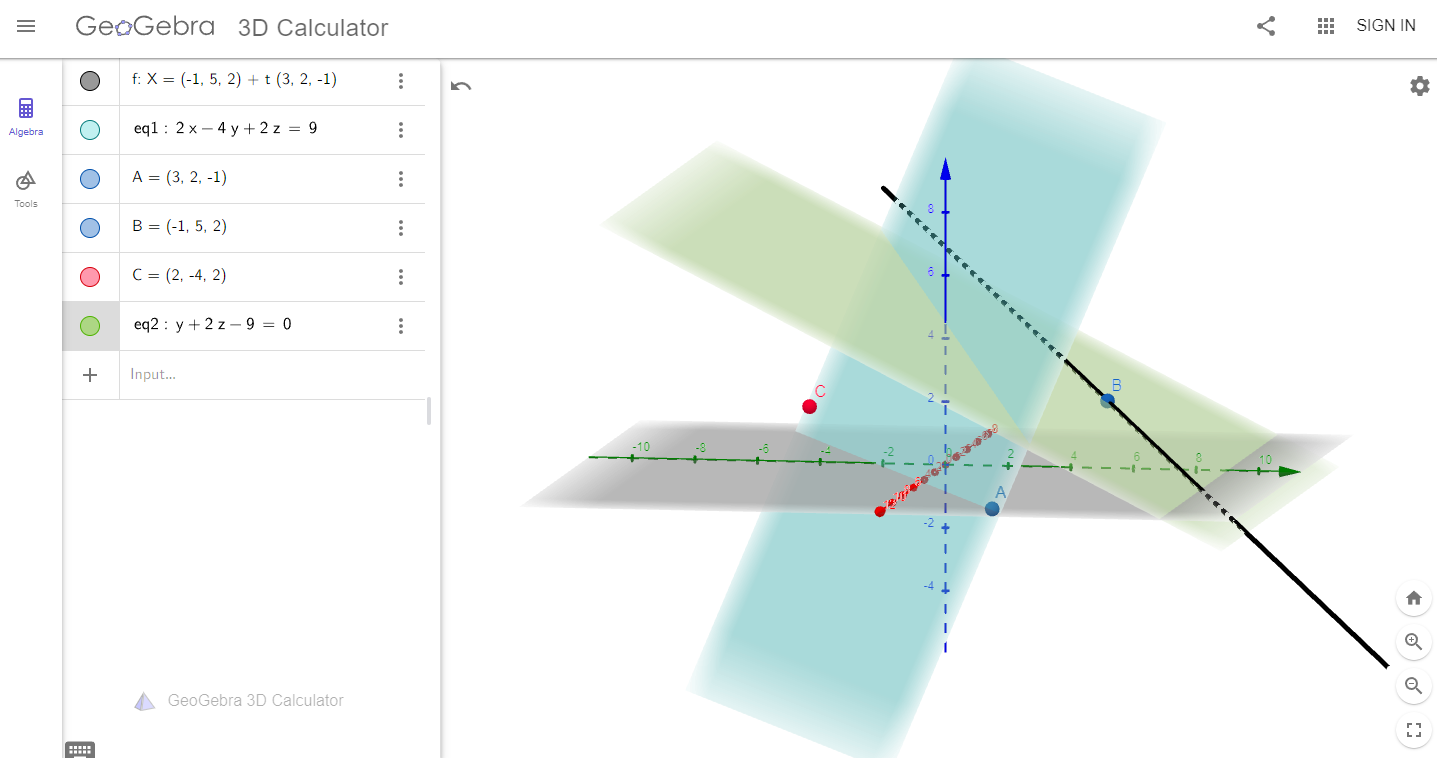
\includegraphics[width=1\textwidth]{sketch-3d-5.png}
\caption{3D Graph of $L \land V_1 \land V_2 \land $} some vectors.
\label{fig:Plane_3D_worked_5}
\end{figure}
































\newpage

\end{document}